\chapter{Clustering}
\section{What is clustering?}
\textbf{Clustering} is the task of dividing the population or data points into a number of groups 
such that data points in the same groups are more similar to other data 
points in the same group and dissimilar to the data points in other groups. 
It is basically a collection of objects 
on the basis of similarity and dissimilarity between them.\par

Usually, we can represent the training set as $\{x^{(1)}, x^{(2)}, x^{(3)}, \cdots, x^{(m)}\}$,
where $x^{(i)}$ is a feature vector representing the $i^{th}$ training example.
For example if the number of features $n$ is 2, then $x^{(i)}$ is a 2D vector.
We can draw the scatter plot of the training set, 
and we can see that the training set is divided into several clusters.

\begin{center}
\includegraphics*[width=0.8\textwidth]{images/km1}
\end{center}

\section{K-means Algorithm}
\subsection*{K-means Intuition}
The K-means algorithm is a method to automatically cluster similar data examples together.
Here is the steps of the K-means algorithm:
\begin{thmbox}{Simplified K-means Algorithm}{kmeans}
    \begin{description}
        \item[step 1]: Assign each data point to the closest centroid.
        \item[step 2]: Compute the new centroids by averaging the data points assigned to each centroid.
    \end{description}
\end{thmbox}

\subsection*{Algorithm}
\begin{thmbox}{K-means Algorithms}{kmeans}
    \begin{enumerate}
        \item Randomly initialize the $K$ cluster centroids $\mu_1, \mu_2, \cdots, \mu_K$.
        \item Repeat \{
        \item[] \hspace*{1em} for $i = 1$ to $m$ \{
        \item[] \hspace*{2em} $c^{(i)}$ := index of cluster centroid closest to $x^{(i)}$
        \item[] \hspace*{1em} \}
        \item[] \hspace*{1em} for $k = 1$ to $K$ \{
        \item[] \hspace*{2em} $\mu_k$ := average of points in cluster k
        \item[] \hspace*{1em} \} 
        \item[] \}
    \end{enumerate}
    \tcblower
    \begin{notebox}
        \begin{itemize}
            \item $K$ is the number of clusters
            \item $m$ is the number of training examples
            \item $n$ is the number of features
            \item $c^{(i)}$ is the index of the centroid that is closest to $x^{(i)}$
            \item $\mu_k$ is the location of the $k^{th}$ centroid
        \end{itemize}
        \tcblower
        \hspace{2em} If one cluster centroid is not assigned any data points,
        then usually let K = K - 1 and repeat the algorithm.
        But if it is requested to keep K clusters, then you can randomly initialize the centroid again.
    \end{notebox}
\end{thmbox}

\section{Optimization Objective}
\begin{thmbox}{Cost function of K-means}{ck}
    \begin{itemize}
        \item $c^{(i)}$ := index of cluster centroid which example $x_{(i)}$ is currently assigned to.
        \item $\mu_k$ := cluster centroid $k$.
        \item $\mu_{c^{(i)}}$ := cluster centroid of cluster to which example $x^{(i)}$ has been assigned. 
    \end{itemize}
    the $\mu_k$ and $\mu{c^{(i)}}$ are both $n$-dimensional vectors.
    \tcblower
    \begin{equation}
        J(c^{(1)}, \cdots, c^{(m)}, \mu_1, \cdots, \mu_K) = \frac{1}{m} \sum_{i=1}^{m} \Vert x^{(i)} - \mu_{c^{(i)}}\Vert ^2
    \end{equation}
\end{thmbox}

\begin{notebox}
    \hspace{1em}Our goal is to find the $c^{(1)}, \cdots, c^{(m)}, \mu_1, \cdots, \mu_K$ to minimize $J$.\par
    \hspace{1em}According to the K-means algorithm, first step is to assign each data point to the closest centroid.
    In this procedure, we minimize $J$ with respect to $c^{(1)}, \cdots, c^{(m)}$ 
    while remains the $\mu_1, \cdots, \mu_K$ fixed.\par
    \hspace{1em}The second step is to compute the new centroids by averaging the data points assigned to each centroid.
    In this procedure, we minimize $J$ with respect to $\mu_1, \cdots, \mu_K$, 
    while remains the $c^{(1)}, \cdots, c^{(m)}$ fixed.
\end{notebox}

\begin{exbox}{Moving the centroid}{mc}
    \includegraphics*[width=\textwidth]{images/km2}
\end{exbox}

The K-means algorithm is guaranteed to converge to a local optimum. And after each iteration, 
the cost function $J$ will always decrease. But the K-means algorithm may not converge to the global optimum.
Even delt with not well-separated clusters, we can also apply the K-means algorithm to separate them.
\section{Random Initialization}

\begin{notebox}
\begin{enumerate}
    \item Choose $K<m$. 
    \item Randomly pick $K$ training examples.
    \item Set $\mu_1, \mu_2, \cdots, \mu_K$ equal to these $K$ examples.
\end{enumerate}
\tcblower
\begin{itemize}
    \item The K-means algorithm can converge to different solutions depending on the initial setting of the centroids.
    \item To solve this problem, we can run the K-means algorithm multiple times with different random initializations.
    \item We can then choose the clustering that gave us the lowest cost.
\end{itemize}
\end{notebox}

\begin{center}
    \includegraphics*[width=\textwidth]{images/km3}
\end{center}

\begin{thmbox}{Random Initialization}{ri}
    \begin{enumerate}
        \item[] For $i = 1$ to $100$ \{
        \item[] \hspace*{1em} Randomly initialize $K$-means.
        \item[] \hspace*{1em} Run K-means. Get $c^{(1)}, \cdots, c^{(m)}, \mu_1, \cdots, \mu_K$.
        \item[] \hspace*{1em} Compute cost function (distortion)$J(c^{(1)}, \cdots, c^{(m)}, \mu_1, \cdots, \mu_K)$. 
        \item[] \}
        \item[] Pick clustering that gave lowest cost $J$.
    \end{enumerate}
    \tcblower
    \hspace*{1em}The training times is often set to 50 - 1000.
\end{thmbox}

\section{Choosing the Number of Clusters}
\subsection*{Elbow Method}

\begin{enumerate}
    \item Run K-means for a range of values of $K$.
    \item For each value of $K$, calculate the distortion.
    \item Plot the distortion against the number of clusters $K$.
    \item The elbow point is the point where the distortion starts to decrease more slowly.
\end{enumerate}

\begin{center}
    \includegraphics*[width=\textwidth]{images/km4}
\end{center}

\begin{notebox}
    \hspace{2em}The elbow point is not clear most of the time.\par
    \hspace{2em}And don't always need to choose the number of clusters that minimize the distortion.
    Because as the number of clusters increases, the distortion will decrease all the time.
\end{notebox}

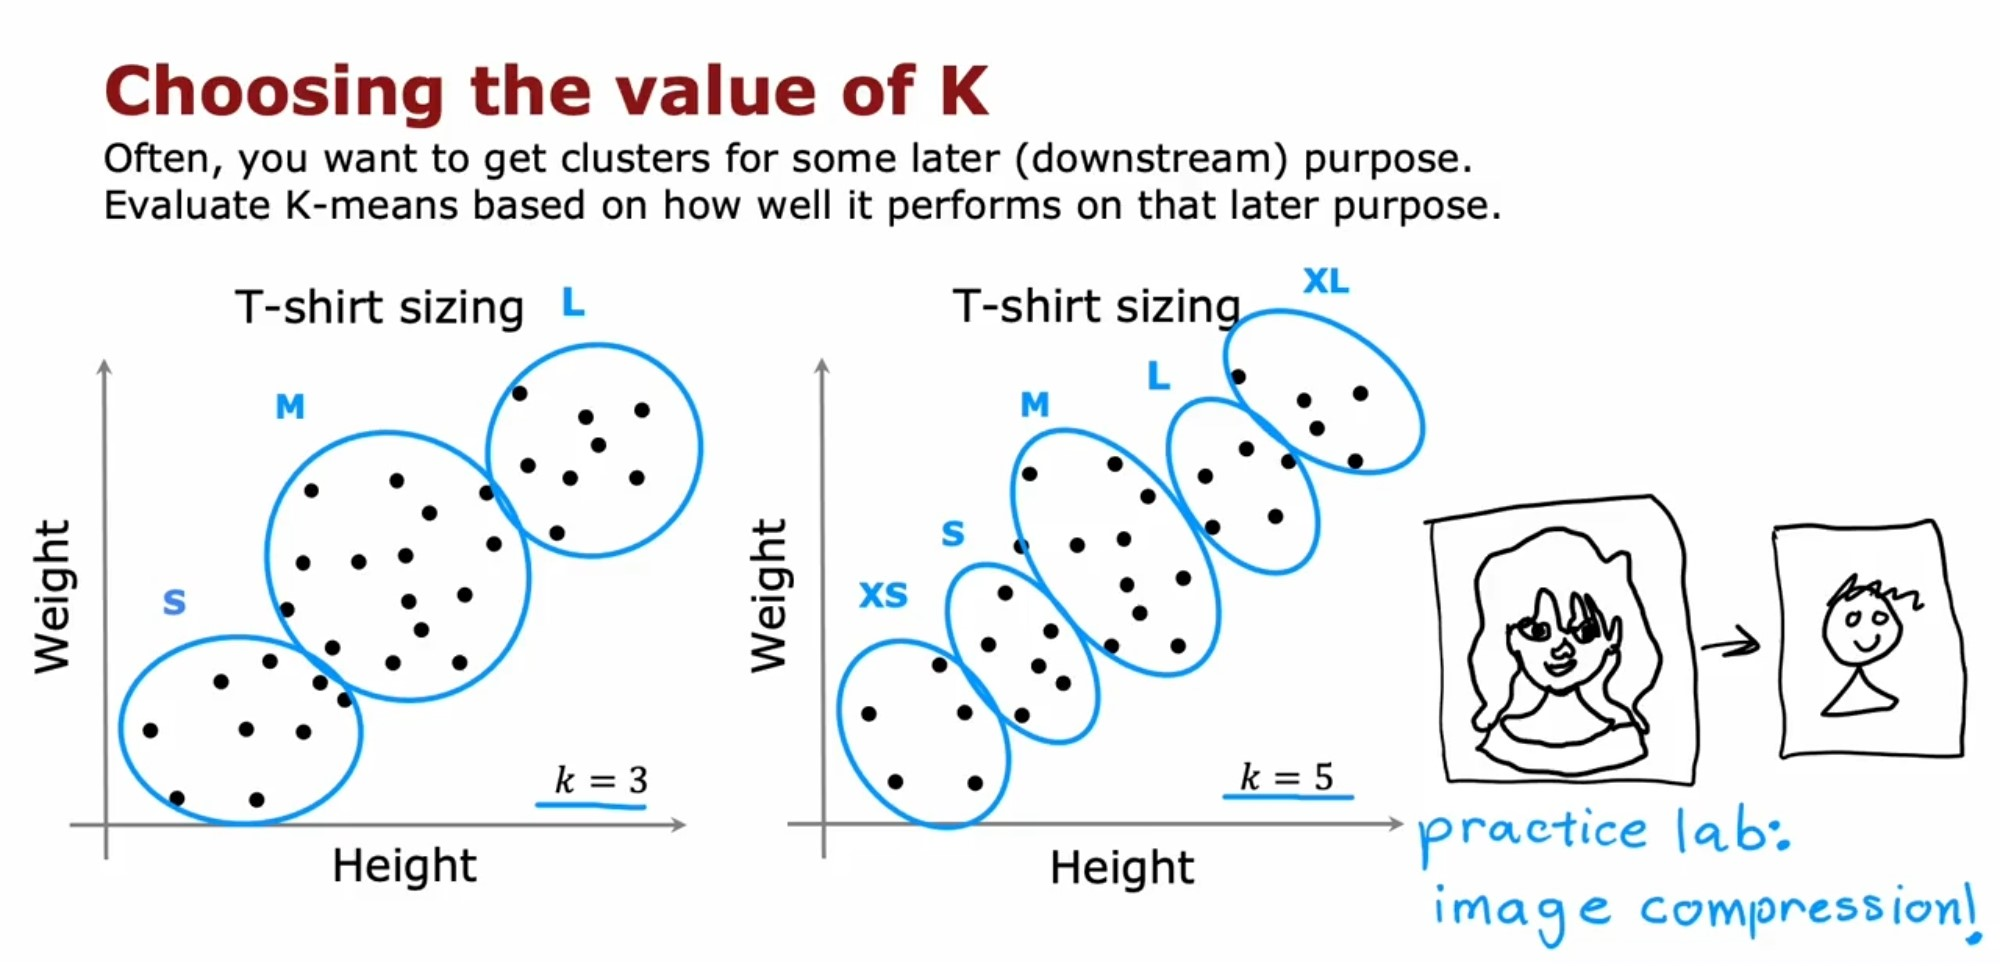
\includegraphics[width=\textwidth]{images/km5}

\section{K-means from Scratch}
\textbf{file name: kmeans.py}
\amzinputcode{python}{codes/kmeans.py}